\kap{NN-scattering up to 1 GeV}\label{chap:NN-scattering up to 1 GeV}


There can be some inelasticity from Bremsstrahlung ($N+N\to N+N+\gamma)$ in the scattering.
This term is small and will diaper when we neglect the electromagnetic force. Larger inelasticity
are entering the picture for lab energies about 300 MeV.
This is due to
fact that at 300 MeV, nucleons have enough energy to create a free $\pi$-meson ($N+N\to N+N+\pi$).
At higher
energies creations of other mesons will also enter the process.
Creation of such mesons will also have an effect on the phase shifts.

At 600 MeV creation of two $\pi$-mesons are possible, but at this energy another important factor to the inelasticity
can arrive.
This is due to the the excitations of one the nucleons into $\triangle$(1232).
%If the state is virtually excited to $\triangle$, the virtual state can fall back to the ground state (N). In this process, 
%there will be created a free meson in the process.
%This has such a big effect on the inelasticity since it doesn't only slow down the speed of the nucleons, which is what the
%$\pi$-mesons does. $\triangle$ excitation also remove one nucleon in the process.
%But the biggest contribution to the
%inelasticity at higher energies is the 2 mesons exchange that can change one of the incoming nucleons. At
%lab energies around 600 MeV we can get the 2 $\pi$ exchange through the process
$N+N\to N+\triangle$. 
Because of isospin addition rules, this process is only possible with a two nucleon state with isospin $I=1$.
%Where $\triangle$ has the same barion number and the total isospin as the nucleon N it replaced.

If the state is virtually excited to $\triangle$, the virtual state can fall back to the ground state (N). In this process,
there will be created a free meson in the process.

There exist four $\triangle$-barions
and they come from the isospin-$\frac{2}{3}$ barion group.
They can be expressed in terms of quarks as $\triangle^-={\textrm{ddd}}(I_3=-3/2)$,\;$\triangle^-=\textrm{udd}(I_3=-1/2)$,
\;$\triangle^-={\textrm{uud}}(I_3=1/2)$ and $\triangle^{++}={\textrm{uuu}}(I_3=3/2)$. Where $I_3$ is related to the particles
electrical charge. This quatety is concerved since the charge is conseved.
%If we assume that the isospin is a good quantum number. i.e. we neglect the decays done by the
%electromagnetic and the week force.
For the barion dublet we have $n$($I_3=-1/2$) and $p$($I_3=1/2$).
%
%We therefor have that $p+p\to p+\triangle^{+}$ is one of the possible $\triangle$ excitations.
%
At energies above 1,2 GeV we can get double $\triangle$ excitations ($N+N\to \triangle+\triangle$).
This process is posible for states with both isospin 0 and 1.
If we want to include the inelasticety caused by a one or a two 
$\triangle$ exitation using a real potential like the "bonn B"-potential
, we have to include the width $im^{{\text imag}}_\triangle$ 
of the $\triangle$-barions in the propagators of the coupled $\LS$ equation.
This width (self-energy) will be a complex componet
of the energy/mass. 
\begin{equation}
m_\triangle=m^{{\text real}}_\triangle+im^{{\text imag}}_\triangle
\end{equation}
The real part will be the same as before. 







\section{Coupled Channels And The "nna13"-Potential}
If we want to include the viretual $\triangle$-excitations, we need
to include two mesons exchange deagrams to the OBEP moddel. This is shown in
fig~\ref{figVnna13}, where only the creation of $\pi$ and $\rho$ are included.
BEDREEEEEEEEThe self-energy model is
equivalent to three body Feynman diagrams were mesons are emitted in the process.
This will give a coupled
channel vertion of the $\LS$ equation, which is
\begin{eqnarray}
{T}_{NN,NN}=V_{NN,NN}&-&\int d^3k\frac{V_{NN,NN}{T}_{NN,NN}}{\varepsilon_{NN}-\varepsilon^0_{NN}}
-\int d^3k\frac{V_{NN,N\triangle}{T}_{N\triangle,NN}}{\varepsilon_{N\triangle}-\varepsilon^0_{NN}}\nonumber\\
&-&\int d^3k\frac{V_{NN,\triangle\triangle}{T}_{\triangle\triangle,NN}}{\varepsilon_{\triangle\triangle}-\varepsilon^0_{NN}} 
\end{eqnarray}
where  
\begin{eqnarray}
{T}_{N\triangle,NN}=V_{N\triangle,NN}&-&\int d^3k\frac{V_{N\triangle,NN}{T}_{NN,NN}}{\varepsilon_{NN}-\varepsilon^0_{NN}}
-\int d^3k\frac{V_{N\triangle,NN}{T}_{N\triangle,NN}}{\varepsilon_{N\triangle}-\varepsilon^0_{NN}}\nonumber\\
&-&\int d^3k\frac{V_{N\triangle,\triangle\triangle}{T}_{\triangle\triangle,NN}}{\varepsilon_{\triangle\triangle}-\varepsilon^0_{NN}}
\end{eqnarray}
and all the other ${T}_{xx,xx}$ are calculated similary. To calculate these equations we need to have an expression for
all the different potentials $V_{xx.xx}$ like $V_{NN,N\triangle}$ and $V_{NN,\triangle\triangle},\cdots$. 
\begin{equation}
\varepsilon_{N\triangle}=E_{{\text N}}+E_\triangle
\end{equation}
where
\begin{equation}
{{\text E}}_{{\triangle}} =\frac{k^2}{2m_{{\triangle}}}+m_{{\triangle}}
\end{equation}
,
\begin{equation}
{{\text E}}_{{\text N}} =\frac{k^2}{2m_{{\text N}}}+m_{{\text N}}
\end{equation}
and the on-shell energy is
\begin{equation}
\varepsilon^0_{NN}=2\bigg(\frac{q^2_0}{2m_{{\text N}}}+m_{{\text N}}\bigg)
\end{equation}

To calculate all the coupled channels is a pretty lenthy task. Since the one $\triangle$-excitation
is much more important for the inelastic system below 1 GeV, one can make the coupled channel problem easier by
neglecting the double $\triangle$-excitations, or
%instead of doing all this, 
one can also make use of the complex
potentials all ready on the marked. Machleidts "nna13"-potential for 
example. This potential is relatively good up to 1 GeV, and
includes both one and two virtual $\triangle$ excitations. 
%This self-energy model is
%equivalent to three body Feynman diagrams were mesons are emitted in the process. 
%The propagator between a 
%excited $\triangle$ and a N is implemented in nna13, and is on the form
The nna13 potential has been written so that one can use the uncoupled $\LS$ equation
with the same propagator as in the OBE potential
\begin{equation}
{{\text G(E)}}=\frac{1}{\varepsilon_{NN}-\varepsilon^0_{NN}}
%\frac{1}{z_0-E_\triangle-E_{{\text N}}}
\end{equation}
%where 
%\begin{equation}
%{{\text E}}_{{\triangle}} =\frac{k^2}{2m_{{\triangle}}}+m_{{\triangle}} 
%\end{equation}
%,
%\begin{equation}
%{{\text E}}_{{\text N}} =\frac{k^2}{2m_{{\text N}}}+m_{{\text N}} 
%\end{equation}
%and the on-shell energy is
%\begin{equation}
%z_0=2\bigg(\frac{q^2_0}{2m_{{\text N}}}+m_{{\text N}}\bigg)  
%\end{equation}
%The propagator in the  $\LS$ equation will be the same as before, since we still the same NN-propagator.
%One can therefor explane the small
%inelasticity at low enegies, by the small self-energies of N.
At higer energies also effects like N* (Roper resonance) has to be included.

The one boson exchange diagrams of the nna13 potential is build up as shown in fig~\ref{figVnna13},
where also the two exchange diagrams of the $\triangle$ excitation are included.
The nna13 potential also include the cdbonn package (\ref{cdbonn}), which means that the nna13 potential is also 
including the charge dependece in the scattering. This way
the nna13 potential is fitted better to the experimental data than a plane OBE potential. 

This is based on a field theoretic model, where only the lowest $\triangle$/(N$\pi$) excitations are taken into account.
The fictive $\sigma$-meson is taken apart, so we can seperate the processes that causes creation of the lightest mesons.
Of these new $\triangle$ diagrams, the 2$\pi$ exchanges are 
the most important effect.
Also the $\pi\rho$ and $\rho\rho$ exchange diagrams are important. 
From OBEP the diagrams of one and two $\triangle$ excitation
are removed from the $\sigma$. The new $\sigma'$ is therefor a little different from the $\sigma$ from the OBE.
These changes are included in the nna13 potential to describe the effect of the inelastic part of the scattering.
\nl
\begin{figure}{}
%\begin{center} 
\begin{picture}(330,95)(0,0)
\Text(5,50)[l]{$V_{NN} =$}
\Line(50,5)(50,95)
\Vertex(50,50){2}
\DashLine(50,50)(150,50){5}
\Line(150,5)(150,95)
\Vertex(150,50){2} 
\Text(100,40)[c]{$\pi,\eta,\rho,\omega,\delta,\sigma '$} 
\Text(160,50)[l]{$+$}
\Line(180,5)(180,95)
\Boxc(182,50)(4,40)
\Text(190,50)[l]{$\Delta$}
\DashLine(182,70)(240,70){5}
\DashLine(182,30)(240,30){5}
\Line(240,5)(240,95)
\Text(210,80)[c]{$\pi,\rho$}
\Text(210,20)[c]{$\pi,\rho$}
\Text(250,50)[l]{$+$} 
\Line(270,5)(270,95)
\Boxc(272,50)(4,40)
\Text(280,50)[l]{$\Delta$}
\DashLine(272,70)(330,70){5}
\DashLine(272,30)(330,30){5}
\Text(313,50)[l]{$\Delta$}
\Line(330,5)(330,95)
\Boxc(328,50)(4,40) 
\Text(300,80)[c]{$\pi,\rho$}
\Text(300,20)[c]{$\pi,\rho$}
\end{picture} 
\caption{\label{figVnna13} \sl The three body diagram of the OBE part of the nna13 potential and the two meson exchange
$\triangle$-excitation diagrams. All of higer order diagrams have been neglected.
Solid lines denotes nucleons.
The first diagram on the left hand side is a one meson exchange diagram, and the two others are excited states
of the two meson exchange diagrams.} 
%\end{center}
\end{figure}

The fig~\ref{figVnna13}
is a three body equation. As mentioned before nna13 uses a coupled two-body channel model which is almost equivalent to
the three body equations.
LAG NY FIGUR!!!!!!!!!!!!!!!!!!!!
\nl
The results of the first phase shifts and inelasticities with the nna13 potential are plotted in \ref{fig:hiEnergy}. 
From these data one can calculate the cross section. The total cross section($\sigma$) will be dependent on all the partial waves. 
However the cross section calculated from the phase shifts converges. The importance of
the phase shifts and inelasticity as J increases are shown in tab~\ref{tabcrossel} and tab~\ref{tabcrossinel},
where the program "obs.f" has been used.

\begin{table}[!hbp]
\begin{tabular}{|l|c|c|c|c|c|}
\hline
& \multicolumn{5}{|c|}{$\sigma_{NN-elastic}$ $[mb]$}\\
\hline
$T_{lab}$& { $J_{max}=3$}  & { $J_{max}=10$} & { $J_{max}=20$} & $J_{max}=80$ & Experimental\\
\hline
200 MeV&40.254595&41.849377 &41.851221  &41.851221 &42.78\\
\hline
%300 MeV &35.036848 & & & &32.40\\
%\hline
400 MeV&29.286240&32.212076 &32.228529  &32.228552 &32.40\\
\hline
%500 MeV &30.310964 & & & &26.25\\ 
%\hline
600 MeV&24.781240&28.080876 &28.120242  &28.120412 &29.54\\
%\hline
%700 MeV &26.083066 & & & &\\
\hline
800 MeV&21.486933&24.551982 &24.614851  &24.615376 &26.25\\
%\hline
%900 MeV &23.598118 & & & &\\
\hline
1000 MeV&20.521614&23.093538 &23.177359 & 23.178458 &23.29\\ 
\hline
\end{tabular}
\caption{
\label{tabcrossel}
\sl Total elastic cross section from np scattering using the nna13 potential and all the partial waves up to $J_{max}$. 
Experimental values \cite{PRC62faseskift3GeV}  are also included}
\end{table}
%
%
\begin{table}[!hbp]
\begin{tabular}{|l|c|c|c|c|c|}
\hline
& \multicolumn{5}{|c|}{$\sigma_{NN-elastic}$ $[mb]$}\\
\hline
$T_{lab}$& $J_{max}=3$  & $J_{max}=10$  & $J_{max}=20$ & $J_{max}=80$ & Experimental\\
\hline
200 MeV&0.000000&0.000000 &0.000000  &0.000000 &0.0000\\
%\hline
%300 MeV &0.006844 & & & &\\
\hline
400 MeV&0.477711&0.518062 &0.518062  &0.518062 &0.6947\\
%\hline
%500 MeV &2.429705 & & & &\\
\hline
600 MeV&6.036612&6.706089 &6.707221  &6.707221 &6.479\\
%\hline
%700 MeV &9.410750 & & & &\\
\hline
800 MeV&8.879003&11.032602 &11.040103  &11.040103 &12.37\\
\hline
%900 MeV &12.442983 & & & &\\
%\hline
1000 MeV&9.815736&13.053151&13.074315  &13.074315 &15.45\\
\hline
\end{tabular}
\caption{
\label{tabcrossinel}
Total inelastic cross section from np scattering using the nna13 potential and all the partial waves up to $J_{max}$.
Experimental values \cite{PRC62faseskift3GeV}  are also included}
\end{table}


%\begin{equation}\label{eq:probforelastic}
%N+N\to N+N
%\end{equation}
%This is the elastic process. All the other processes are inelastic. $|\eta_l|^2$ can therefor be interpreted as the
%probability of elastic scattering (\ref{eq:probforelastic}). This definition of
%inelasticity does not contain any information about the relation of all the other inelastic processes. Like
%the probability of one pion or two pion creation in the scattering.


For higher energy scattering, we also have to include the substructure of the Hadrons. This model has to be based on quarks, 
and the OBE model is no longer sufficient to describe the NN-scattering process. 



\begin{flushleft} 
\begin{figure}%\label{fig:hiEnergy}
%\centering
\begin{flushleft} 
\includegraphics[height=20cm,width=18cm]{figd85_alt1.ps} 
\end{flushleft}  
%\caption{\state{1}{S}{0} phase shifts for a box Potential, a parameterized potential, the Bonn B potential and
%experimental data ~\cite{PRC48faseskift350MeV}. How the potentials are build up
%will be explained later.}
\end{figure}
\end{flushleft}

\begin{flushleft}
\begin{figure}%\label{fig:hiEnergy}
%\centering
\begin{flushleft}
\includegraphics[height=20cm,width=18cm]{figd85_alt2.ps}
\end{flushleft}
%\caption{\state{1}{S}{0} phase shifts for a box Potential, a parameterized potential, the Bonn B potential and
%experimental data ~\cite{PRC48faseskift350MeV}. How the potentials are build up
%will be explained later.}
\end{figure}
\end{flushleft}

\begin{figure}%\label{fig:hiEnergy}  
%\centering
\begin{flushleft}
\includegraphics[height=20cm,width=18cm]{figd85_alt3.ps}
\end{flushleft}
%\caption{\state{1}{S}{0} phase shifts for a box Potential, a parameterized potential, the Bonn B potential and
%experimental data ~\cite{PRC48faseskift350MeV}. How the potentials are build up
%will be explained later.}
\end{figure}

\begin{figure}%\label{fig:hiEnergy}
%\centering
%\begin{flushleft}
\includegraphics[height=20cm,width=18cm]{figd85_alt4.ps}
%\end{flushleft}
\caption{\label{fig:hiEnergy} Theoretical phase shifts and inelasticities for a OBE potential ("cd-bonn")
that includes N-$\triangle$ and $\triangle$-$\triangle$ box diagrams. This complex potential is called "nna13"
and was written by R. Machleidt in 2000. The dots are experimental values. Where the black dots are taken 
from \cite{PRC48faseskift350MeV}, and
the white dots from \cite{PRC62faseskift3GeV}}
\end{figure}
